\section{Applied Optimization}
\label{sec:app-opt}

We have used derivatives to help find the maxima and minima of some functions given by equations, but it is very unlikely that someone will simply hand you a function and ask you to find its extreme values. More typically, someone will describe a problem and ask your help in maximizing or minimizing something. What is the largest volume package which the post office will take? What is the quickest way to get from here to there? What is the least expensive way to accomplish some task? In this section, we'll discuss how to find these extreme values using calculus.

\subsection{Applications of Extrema}
\begin{example}
The manager of a garden store wants to build a 600 square foot rectangular enclosure on the store's parking lot in order to display some equipment. Three sides of the enclosure will be built of redwood fencing, at a cost of \$7 per running foot. The fourth side will be built of cement blocks, at a cost of \$14 per running foot. Find the dimensions of the least costly such enclosure.
\end{example}

The process of finding maxima or minima is called {\bf optimization}\index{Optimization}. The function we're optimizing is called the {\bf objective function}\index{Objective function}\index{Function!objective} (or objective equation). The objective function can be recognized by its proximity to superlatives (greatest, least, highest, farthest, most, etc.). Look at the garden store example; the cost function is the objective function.

In many cases, there are two (or more) variables in the problem. In the garden store example again, the length and width of the enclosure are both unknown. If there is an equation that relates the variables we can solve for one of them in terms of the others, and write the objective function as a function of just one variable. Equations that relate the variables in this way are called {\bf constraint equations} or simply {\bf constraints}\index{Constraints}. The constraint equations are always equations, so they will have equals signs. For the garden store, the fixed area relates the length and width of the enclosure. This will give us our constraint equation.

\paragraph*{Applied Optimization Problem Technique}
  \begin{enumerate}
      \item Translate the English statement of the problem line by line into a picture (if that applies) and into math. This is often the hardest step!
      \item Identify the objective function. Look for words indicating a largest or smallest value.
      \begin{enumerate}[label=(\alph*)]
        \item If you seem to have two or more variables, find the constraint equation. Think about the English meaning of the word constraint, and remember that the constraint equation will have an equals sign.
        \item Solve the constraint equation for one variable and substitute into the objective function. Now you have an equation of one variable.
      \end{enumerate}
      \item Use calculus to find the optimum values. (Take derivative, find critical points, test. Don't forget to check the endpoints!)
      \item Look back at the question to make sure you answered what was asked. Translate your number answer back into English.
    \end{enumerate}

\begin{example}
The manager of a garden store wants to build a 600 square foot rectangular enclosure on the store's parking lot in order to display some equipment. Three sides of the enclosure will be built of redwood fencing, at a cost of \$7 per running foot. The fourth side will be built of cement blocks, at a cost of \$14 per running foot. Find the dimensions of the least costly such enclosure.

\begin{solution} First, translate line by line into math and a picture:

\begin{itemize}
  \item The manager of a garden store wants to build a 600 square foot rectangular enclosure on the store's parking lot in order to display some equipment.

  We will give variable names to the unknown quantities. We're given a rectangular area of 600 ft$^2$. Since area is length times width, let $x$ be the width of the enclosure and let $y$ its length, the length of the side made of blocks. Then area is $A(x, y) = xy = 600$. This is a constraint. Since length and width must be positive, we have two more constraints: $x\ge 0$ and $y\ge 0$.

  \item Three sides of the enclosure will be built of redwood fencing, at a cost of \$7 per running foot. The fourth side will be built of cement blocks, at a cost of \$14 per running foot.

  A length of $2x+y$ costs \$7 per foot, and the length of $y$ costs \$14 per foot, so cost is
  $C(x, y) = 7(2x+y)+14y = 14x+21y$.

  \item Find the dimensions of the least costly such enclosure.

  Find $x$ and $y$ so that $C(x, y)$ is minimized.
\end{itemize}

\begin{figure}[!ht]
  \centering
    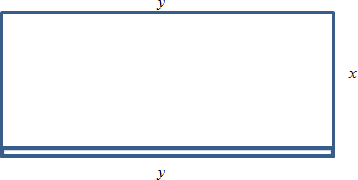
\includegraphics[width=0.4\textwidth]{img/chap3/image090.png}
    %\caption{Visualizing the Second Derivative Test}
    %\label{fig:3-4-2derivtest}
\end{figure}
The objective function is the cost function, and we want to minimize it. As it stands, though, it has two variables, so we need to use the constraint to eliminate one variable. The constraint equation is the fixed area $A=xy=600$. Solve $A$ for $x$ to get $x=\dfrac{600}{y}$, and then substitute into $C(x, y)$:
$$C(y)=14\cdot\dfrac{600}{y}+21y=\dfrac{8400}{y} + 21y \enspace .$$
Now we have a function of just one variable, so we can find the minimum using calculus.

$$C'(y)=-\dfrac{8400}{y^2}+21$$
$C'(y)$ is undefined for $y=0$, so we'll solve $C'=0$ for $y$.
\begin{align*}
  -\frac{8400}{y^2}+21 &= 0\\
  21 &= \frac{8400}{y^2} \\
  21 y^2 &= 8400\\
  y^2 &= 400\\
  y &= \pm 20
\end{align*}
So cost is optimized when $y=20$ or $y=-20$, but of the three critical numbers, only $y=20$ makes sense (since it is within the constraints).

Test $y=20$ (here we chose the second derivative test):
$$C''(20)=\dfrac{16800}{y^3}>0 \enspace ,$$
so this is a local minimum.

Since this is the only critical point in the domain, this must be the global minimum. Going back to our constraint function, we can find that when $y=20$, $x=30$. The dimensions of the enclosure that minimize the cost are 20 feet by 30 feet.
\end{solution}\end{example}

When trying to maximize their revenue, businesses also face the constraint of consumer demand. While a business would love to see lots of products at a very high price, typically demand decreases as the price of goods increases. In simple cases, we can construct that demand curve to allow us to maximize revenue.

\begin{example}
A concert promoter has found that if she sells tickets for \$50 each, she can sell 1200 tickets, but for each \$5 she raises the price, 50 less people attend. What price should she sell the tickets at to maximize her revenue?

\begin{solution} We are trying to maximize revenue, and we know that $R=pq$, where $p$ is the price per ticket, and $q$ is the quantity of tickets sold.

The problem provides information about the demand relationship between price and quantity -- as price increases, demand decreases. We need to find a formula for this relationship. To investigate, let's calculate what will happen to attendance if we raise the price in Table \ref{tab:3-6-tickets}.

\begin{table}[ht!]
    \centering
    \begin{tabular}{l*{4}{r}}
    \toprule
    Price, $p$    &	50    &	55    &	60    &	65 \\
    \midrule
    Quantity, $q$	& 1200  &	1150  &	1100  &	1050\\
    \bottomrule
    \end{tabular}
    \caption{Demand for tickets as a function of price.}
    \label{tab:3-6-tickets}
\end{table}
You might recognize this as a linear relationship. We can find the slope for the relationship by using two points:
$$m = \frac{1150-1200}{55-50}=-\frac{50}{5}=-10 \enspace .$$
You may notice that the second step in that calculation corresponds directly to the statement of the problem: the attendance drops 50 people for every \$5 the price increases.

Using the point-slope form of the line, we can write the equation relating price and quantity:
$$q-1200=-10(p-50) \enspace .$$
Simplifying to slope-intercept form gives the demand equation
$$q=1700-10p \enspace .$$
Substituting this into our revenue equation, we get an equation for revenue involving only one variable:
$$R=pq=p(1700-10p)=1700p-10p^2 \enspace .$$
Now, we can find the maximum of this function by finding critical numbers. $R'(p)=1700-20p$, so $R'(p)=0$ when $p=85$.

Using the second derivative test, $R''(p)=-20<0$ (for any value of $p$), so the critical number is a local maximum. Since it is the only critical number, we can also conclude that $R(85)$ is the global maximum.

The promoter will be able to maximize revenue by charging \$85 per ticket. At this price, she will sell $q(85)=1700-10(85)=850$ tickets, generating $R(85) = \$85\cdot850 = \$72,250$ in revenue.
\end{solution}\end{example}

\subsection{When Marginal Revenue Equals Marginal Cost}
You may have heard before that profit is maximized when marginal cost\index{Marginal cost}\index{Cost!marginal} and marginal revenue\index{Marginal revenue}\index{Revenue!marginal} are equal. Now you can see why people say that! (Even though it's not completely true.)

\begin{example}
Suppose we want to maximize profit.

\begin{solution} Now we know what to do -- find the profit function, find its critical points, test them, etc.

But remember that profit is revenue minus cost: $P(p) = R(p) - C(p)$. So $P'(p) = R'(p)-C'(p)$. That is, the derivative of the profit function is $MR-MC$.

Now let's find the critical points -- those will be where $P'(p) = 0$ or is undefined. $P'(p) = 0$ when $R'(p)-C'(p)=0$, or where $R'(p)=C'(p)$.

In summary, profit has a critical point when marginal revenue and marginal cost are equal.
\end{solution}\end{example}

In all the cases we'll see in this class, profit will be very well behaved, and we won't have to worry about looking for critical points where $P'$ is undefined. But remember that not all critical points are local maxima! Any place where $R'=C'$ could represent a local maximum, a local minimum, or neither.

\begin{example}
A company sells $q$ ribbon winders per year at $\$p$ per ribbon winder. The demand function for ribbon winders is given by: $p=300-0.02q$. The ribbon winders cost \$30 each to manufacture, plus there are fixed costs of \$9000 per year. Find the quantity where profit is maximized.

\begin{solution} We want to maximize profit, but there isn't a formula for profit given. So let's make one. We can find a function for $R = pq$ using the demand function for $p$.
$$R(q)=(300-0.02q)q=300q-0.02q^2 \enspace .$$
We can also find a function for cost, using the variable cost of \$30 per ribbon winder, plus the fixed cost:
$$C(q)=9000+30q \enspace .$$
Putting them together, we get a function for profit:
$$P(q)=R(q)-C(q)=(300q-0.02q^2)-(9000+30q)=-0.02q^2+270q-9000 \enspace .$$
Now we have two choices. We can find the critical points of profit by taking the derivative of $P(q)$ directly, or we can find $R'(p)$ and $C'(p)$ and set them equal. (Naturally, we'll get the same answer either way.)

Let's use $R'(p)=C'(p)$ this time.
\begin{align*}
  R'(p) &= 300-0.04q \\
  C'(p) &= 30 \\
  300-0.04q &= 30 \\
  270 &= 0.04q \\
  q &= 6750
\end{align*}

The only critical point is at $q=6750$. Now we need to be sure this is a local max and not a local min. In this case, we'll look to the graph of $P(q)$ -- it's a downward opening parabola, so this must be a local maximum. And since it's the only critical point, it must also be the global maximum.

Profit is maximized when they sell 6750 ribbon winders.
\end{solution}\end{example}

\subsection{When Average Cost Equals Marginal Cost}
Average cost\index{Average cost}\index{Cost!average} is minimized when average cost equals marginal cost is another saying that isn't quite true; in this case, the correct statement is:
\begin{theorem}
Average Cost has critical points when average cost and marginal cost are equal.
\end{theorem}

Let's look at a geometric argument here. Remember that the average cost is the slope of the diagonal line, the line from the origin to the point on the total cost curve. If you move your clear plastic ruler around, you'll see (and feel) that the slope of the diagonal line is smallest when the diagonal line just touches the cost curve -- when the diagonal line is actually a tangent line -- when the average cost is equal to the marginal cost.

\begin{figure}[!ht]
  \centering
    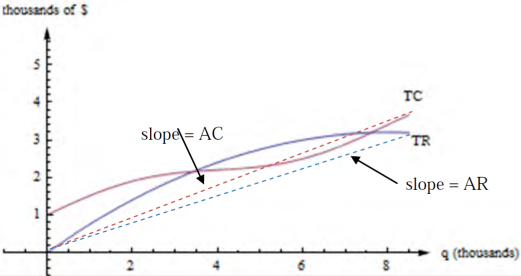
\includegraphics[width=0.4\textwidth]{img/chap3/image113.png}
    %\caption{Visualizing the Second Derivative Test}
    %\label{fig:3-4-2derivtest}
\end{figure}

\subsection{Exercises}
  \begin{enumerate}
    \item A farmer wants to build a pen with two dividers in order to separate elephants, donkeys, and penguins. If 600 ft of fence is available and one side of the pen is bounded by a river and needs no fence since all the animals just happen to have an irrational fear of water, then what is the maximum area that can be enclosed?

    \item A carpenter wants to build a rectangular box with square sides in which to put round things. The material for the bottom costs \$20 per ft$^2$, material for the sides costs \$10 per ft$^2$, and the material for the top costs \$50 per ft$^2$. If the volume of the box must be 5 ft$^3$, then find the dimensions that will minimize the cost (and find the minimum cost).

    \item A knight sees a damsel in distress 3 miles downstream on the opposite side of a straight raging river 0.5 miles wide. The knight can swim at 4 mi/hr and run at 7 mi/hr. At what point on the opposite side should the knight swim in order to reach the distressed damsel as soon as possible?

    \item A box with a square base and open top must have a volume of 32000 cm$^3$. Find the dimensions of the box that will minimize the amount of material needed.

    \item A coffee shop has \$1000 in fixed daily costs and daily costs of \$60 per seat. The daily revenue per seat is \$90 if there are 100 or fewer seats. However, if the seating capacity is more than 100 places, the daily profit per seat will be decreased by \$1 for each additional seat over 100. If the fire marshal will only allow up to 150 seats, what should the seating capacity be in order to maximize the coffee shop’s daily profit?

    \item The total cost in dollars for Alicia to make q oven mitts is given by
    $$C(q) = 64 + 1.5q + 0.01q^2 \enspace .$$
    \begin{enumerate}[label=(\alph*)]
        \item What is the fixed cost?
        \item Find a function that gives the marginal cost.
        \item Find a function that gives the average cost.
        \item Find the quantity that minimizes the average cost.
        \item Confirm that the average cost and marginal cost are equal at your answer to part (d).
      \end{enumerate}

    \item A 5 in.\ $\times$ 8 in.\ piece of paper has a square cut out of each corner (same size from each) and is then folded to make an open-top box. Find the size of the square that will maximize the volume.


    \item Find the area of the largest rectangle that can be inscribed inside an isosceles triangle with side lengths $\sqrt{2}$, $\sqrt{2}$, and $2$.

    \item A right circular cylinder is inscribed in a sphere of radius 6 in. Find the largest possible volume of such a cylinder.
  \end{enumerate}
